% \documentclass[preprint]{elsarticle}
\documentclass[10pt,conference]{ieeeconf}

% \usepackage{lineno,hyperref}
% \modulolinenumbers[5]

\usepackage{mathrsfs}
\usepackage{graphics} % for pdf, bitmapped graphics files
% \usepackage{epsfig} % for postscript graphics files
\usepackage{amsmath} % assumes amsmath package installed
\usepackage{amssymb}  % assumes amsmath package installed
\let\proof\relax
\let\endproof\relax
\usepackage{amsthm}
\usepackage{cite}
\usepackage{bm}
% \usepackage{subfigure}
\usepackage{acronym}
\usepackage{paralist}
\usepackage{float}
\usepackage{color}
\usepackage{epstopdf}
\usepackage{multicol}
\usepackage{tikz}
\usepackage{hyperref}
% \usepackage{subcaption}
\usepackage{graphicx}
% \usepackage{caption}
\usepackage{soul}
\usepackage{mathtools}
\usepackage{siunitx}
\usepackage{empheq}

\makeatletter
\hypersetup{colorlinks=true}
\AtBeginDocument{\@ifpackageloaded{hyperref}
  {\def\@linkcolor{blue}
  \def\@anchorcolor{red}
  \def\@citecolor{red}
  \def\@filecolor{red}
  \def\@urlcolor{red}
  \def\@menucolor{red}
  \def\@pagecolor{red}
\begingroup
  \@makeother\`%
  \@makeother\=%
  \edef\x{%
    \edef\noexpand\x{%
      \endgroup
      \noexpand\toks@{%
        \catcode 96=\noexpand\the\catcode`\noexpand\`\relax
        \catcode 61=\noexpand\the\catcode`\noexpand\=\relax
      }%
    }%
    \noexpand\x
  }%
\x
\@makeother\`
\@makeother\=
}{}}
\makeatother



\newtheorem{Theorem}{Theorem}
\newtheorem{Lemma}{Lemma}
\newtheorem{Problem}{Problem}
\newtheorem{Remark}{Remark}
\newtheorem{Corollary}{Corollary}
\newtheorem{Example}{Example}
\newtheorem{Assumption}{Assumption}
\newtheorem{Definition}{Definition}


\DeclareMathOperator{\rank}{rank}
\DeclareMathOperator{\myspan}{span}
\DeclareMathOperator{\atan2}{atan2}
\DeclareMathOperator{\sgn}{sgn}
\DeclareMathOperator{\sign}{sign}
\DeclareMathOperator{\F}{\mathrm F}
\DeclareMathOperator{\Le}{\mathrm L}
\DeclareMathOperator{\Fp}{\mathrm{F_p}}
\DeclareMathOperator{\R}{\mathbb R}
\DeclareMathOperator{\divergence}{\mathrm{div}}
\DeclareMathOperator{\^T}{^\textrm T}
\DeclareMathOperator{\N}{\textrm N}
\DeclareMathOperator*{\argmax}{arg\,max}
\DeclareMathOperator*{\argmin}{arg\,min}

\newcommand{\bequ}{\begin{eqnarray}}
\newcommand{\eequ}{\end{eqnarray}}
\newcommand{\mT}{^\mathrm{T}}
\newcommand{\rom}{\mathrm}
\def\IR{{\mathbb R}}
\newcommand{\GG}{\text{{\usefont{U}{tx-frak}{m}{n} G}}}
\newcommand{\FF}{\mathcal{F}}
% \newcommand{\SI}{\mathcal{S}}
\newcommand{\LL}{\mathcal{L}}
\newcommand{\ds}{\text{d}s}
\newcommand{\dt}{\text{d}t}
\newcommand{\VV}{\mathcal{V}}
\newcommand{\RI}{\mathcal{R}}

\IEEEoverridecommandlockouts

\def\BibTeX{{\rm B\kern-.05em{\sc i\kern-.025em b}\kern-.08em
    T\kern-.1667em\lower.7ex\hbox{E}\kern-.125emX}}

\begin{document}

\title{\LARGE \bf Adaptive FxT CLF/CBF Sampled-Data Implementation}

\author{Mitchell Black \and Dimitra Panagou
\thanks{
% This paragraph of the first footnote will contain the date on which you submitted your brief for review. It will also contain support  information, including sponsor and financial support acknowledgment. For  example, ``This work was supported in part by the U.S. Department of  Commerce under Grant BS123456.'' 
The authors would like to acknowledge the support of the National Science Foundation award number 1931982.}
\thanks{The authors are with the Department of Aerospace Engineering, University of Michigan, Ann Arbor, MI, USA; \texttt{\{mblackjr, dpanagou\}@umich.edu}.}
}
\maketitle

%%%%%%%%%%%%%%%%%%%%%%%%%%%%%%%%%%%%%%%%%%%%%%%%%%%%%%%%%%%%%%%%%%%%%%%%%%%%%%%%
%********************************** Abstract **********************************%
%%%%%%%%%%%%%%%%%%%%%%%%%%%%%%%%%%%%%%%%%%%%%%%%%%%%%%%%%%%%%%%%%%%%%%%%%%%%%%%%

\begin{abstract}
Abstract belongs here. 
\end{abstract}


%%%%%%%%%%%%%%%%%%%%%%%%%%%%%%%%%%%%%%%%%%%%%%%%%%%%%%%%%%%%%%%%%%%%%%%%%%%%%%%%
%******************************** Introduction ********************************%
%%%%%%%%%%%%%%%%%%%%%%%%%%%%%%%%%%%%%%%%%%%%%%%%%%%%%%%%%%%%%%%%%%%%%%%%%%%%%%%%

\section{Introduction}

Introduction belongs here.

{\color{red}NEED OUTLINE OF PAPER HERE}


%%%%%%%%%%%%%%%%%%%%%%%%%%%%%%%%%%%%%%%%%%%%%%%%%%%%%%%%%%%%%%%%%%%%%%%%%%%%%%%%
%************************* Mathematical Preliminaries *************************%
%%%%%%%%%%%%%%%%%%%%%%%%%%%%%%%%%%%%%%%%%%%%%%%%%%%%%%%%%%%%%%%%%%%%%%%%%%%%%%%%

\section{Mathematical Preliminaries}\label{sec: math prelim}

Mathematical Preliminaries belong here.

% In the rest of the paper, $\mathbb R$ denotes the set of real numbers and $\mathbb R_+$ denotes the set of non-negative real numbers. We use $\|\cdot\|$ to denote the Euclidean norm. We write $\partial S$ for the boundary of the closed set $S$, $\textrm{int}(S)$ for its interior. The Lie derivative of a function $V:\mathbb R^n\rightarrow \mathbb R$ along a vector field $f:\mathbb R^n\rightarrow\mathbb R^n$ at a point $x\in \mathbb R^n$ is denoted as $L_fV(x) \triangleq \frac{\partial V}{\partial x} f(x)$. 

% \subsection{Forward-Invariance of a Set}
% \subsection{Robust Adaptive CBF}
% \subsection{FxT Convergence under Uncertainty}


%%%%%%%%%%%%%%%%%%%%%%%%%%%%%%%%%%%%%%%%%%%%%%%%%%%%%%%%%%%%%%%%%%%%%%%%%%%%%%%%
%**************************** Problem Formulation *****************************%
%%%%%%%%%%%%%%%%%%%%%%%%%%%%%%%%%%%%%%%%%%%%%%%%%%%%%%%%%%%%%%%%%%%%%%%%%%%%%%%%
\section{Problem Formulation}

\noindent We now shift our focus to the problem of safe, adaptive control design for systems subject to nonlinear parametric model uncertainty. Consider a collection of agents modeled via the following dynamical system:

\begin{align}
        \dot z_e &= f_e(z_e) + g(z_e)u \nonumber \\
        \dot z_i &= f_i(z_e,z_1,...,z_N,\phi _i), i \in [1,N] \\
        y_k &= h(z_e,z_1,...,z_N) \nonumber
        % y(t) &= h(z_e,z_1,...,z_N) + v(t) \nonumber
\end{align}

where $z_e$ denotes the state of the ego agent (the subject-agent for which the controller, $u$, is designed), $z_i$ for $i \in [1,N]$ denotes the state of the $i$th agent, $\phi _i$ is a vector of unknown parameters belonging to a nonlinearly parameterized dynamical model for agent $i$, $N$ is the number of agents under consideration, $y_k$ represents the set of state measurements for all agents collected at time $t_k$\iffalse, and $v(t)$ is a zero-mean, white, stationary, Gaussian noise term\fi. We assume also that $f_e: \mathbb{R}^n \rightarrow \mathbb{R}^n$ and $f_i: \mathbb{R}^n \rightarrow \mathbb{R}^n$ for all $i \in [1,N]$ are locally Lipshitz.

Due to the demonstrated efficacy [sources] of the synthesized CLF-CBF-QP control formulation in providing performance guarantees while observing forward-invariance of a safe set, we employ this framework for the purpose of our controller design in the following discussion.

\subsection{Optimization-Based Control Formulation}

\begin{subequations}\label{Adaptive FxT CLF-CBF QP}
\begin{flalign}
    \min_{u,\delta _0,\delta _1,...,\delta _N} \frac{1}{2}\|u-k(x)\|^2 +p_1\delta _0^2 &+ ... +p_N\delta _N^2 +q_0\delta _0 \label{pt_J}\\
    \textrm{s.t.} \; A_{u}u & \leq b_u \label{pt_c}\\
    L_fV(z_e)+L_gV(z_e)u & \leq  \delta _0 - \alpha_1 \max\{0,V(z_e)\}^{\gamma _1} - \alpha_2\max\{0,V(z_e)\}^{\gamma _2} \label{pt_V}\\
    L_fh_{s_1} + L_gh_{s_1}u & \leq \delta _1h_{s_1} \label{pt_S1}\\
    \vdots \nonumber \\
    L_fh_{s_N} + L_gh_{s_N}u & \leq \delta _Nh_{s_N} \label{pt_S2}
\end{flalign}
\end{subequations}

where $u$ represents the control input, $\delta _0$ is a relaxation term on the fixed-time convergence guarantee, and $\delta _1,...,\delta _N$ are slack variables which allow for greater flexibility in control solutions inside of the control-invariant set without violating set-invariance at the boundary. The terms $h_{s_1},...,h_{s_N}$ denote the shorthand for functions $h_{s_1}(z_e,z_1,...,z_N,\phi _1,...,\phi _N),...,h_{s_N}(z_e,z_1,...,z_N,\phi _1,...,\phi _N)$, which are abbreviated for conciseness.

\subsection{Parameter Estimation}
We now address the problem of estimating the unknown parameters belonging to $\phi \in \mathbb{R}^m$. The proposed technique relies on the method of nonlinear multivariate regression. Before proceeding, we need to establish the following assumptions.

\begin{Assumption}
Our ego agent has access to perfect state measurements at discrete time intervals through the measurement model, $y_k$.
\end{Assumption}

\begin{Assumption}
The nonlinearly parameterized model uncertainty belongs to a compact domain, $\phi _i \in \Phi$.
\end{Assumption}

By employing these assumptions, we may estimate the unknown parameters present in the nonlinear dynamical models by solving a nonlinear multivariate regression problem of the following form:

\begin{subequations}\label{Parameter Estimation Regression}
\begin{align}
    \hat{\phi} = \argmin \frac{1}{2} \|\hat{\mu} - \mu (y_{1,...,k},\hat{\phi})\| \label{nl mult reg}\\
    \textrm{s.t.} \; \hat{\phi} &\in \Phi \label{compact}
\end{align}
\end{subequations}

where $\mu$ represents the estimated time-history of the dynamics to which the estimated parameters, $\phi$, are being fit.

The question then becomes, how can we relax the safety requirements given estimates of the behaviors of the other agents in the system?

% \subsection{Decision Barrier Function}




%%%%%%%%%%%%%%%%%%%% Below this is kind of garbage %%%%%%%%%%%%%%%%%%%%%%%%%%%%%

% In this section, we introduce a framework for solving the overtake problem via a {\color{blue}safety estimator} and a FxT CLF-CBF QP subject to bounded, non-vanishing, additive disturbances.

% \subsection{Problem Formulation}
% We consider an Ego car starting behind a slowly-moving, Lead car on a two-lane undivided highway which seeks to overtake the Lead car in a safe, timely manner whilst avoiding oncoming traffic (see Figure \ref{fig:problem setup}). The challenges specific to the problem include lane keeping (maintaining the vehicle's position at the center of the lane), obstacle avoidance (maintaining safe distance from the Lead vehicle and the Oncoming vehicles) within a fixed time, $T$, all while adhering to input constraints.

% \begin{figure}[!ht]
%     \centering
%         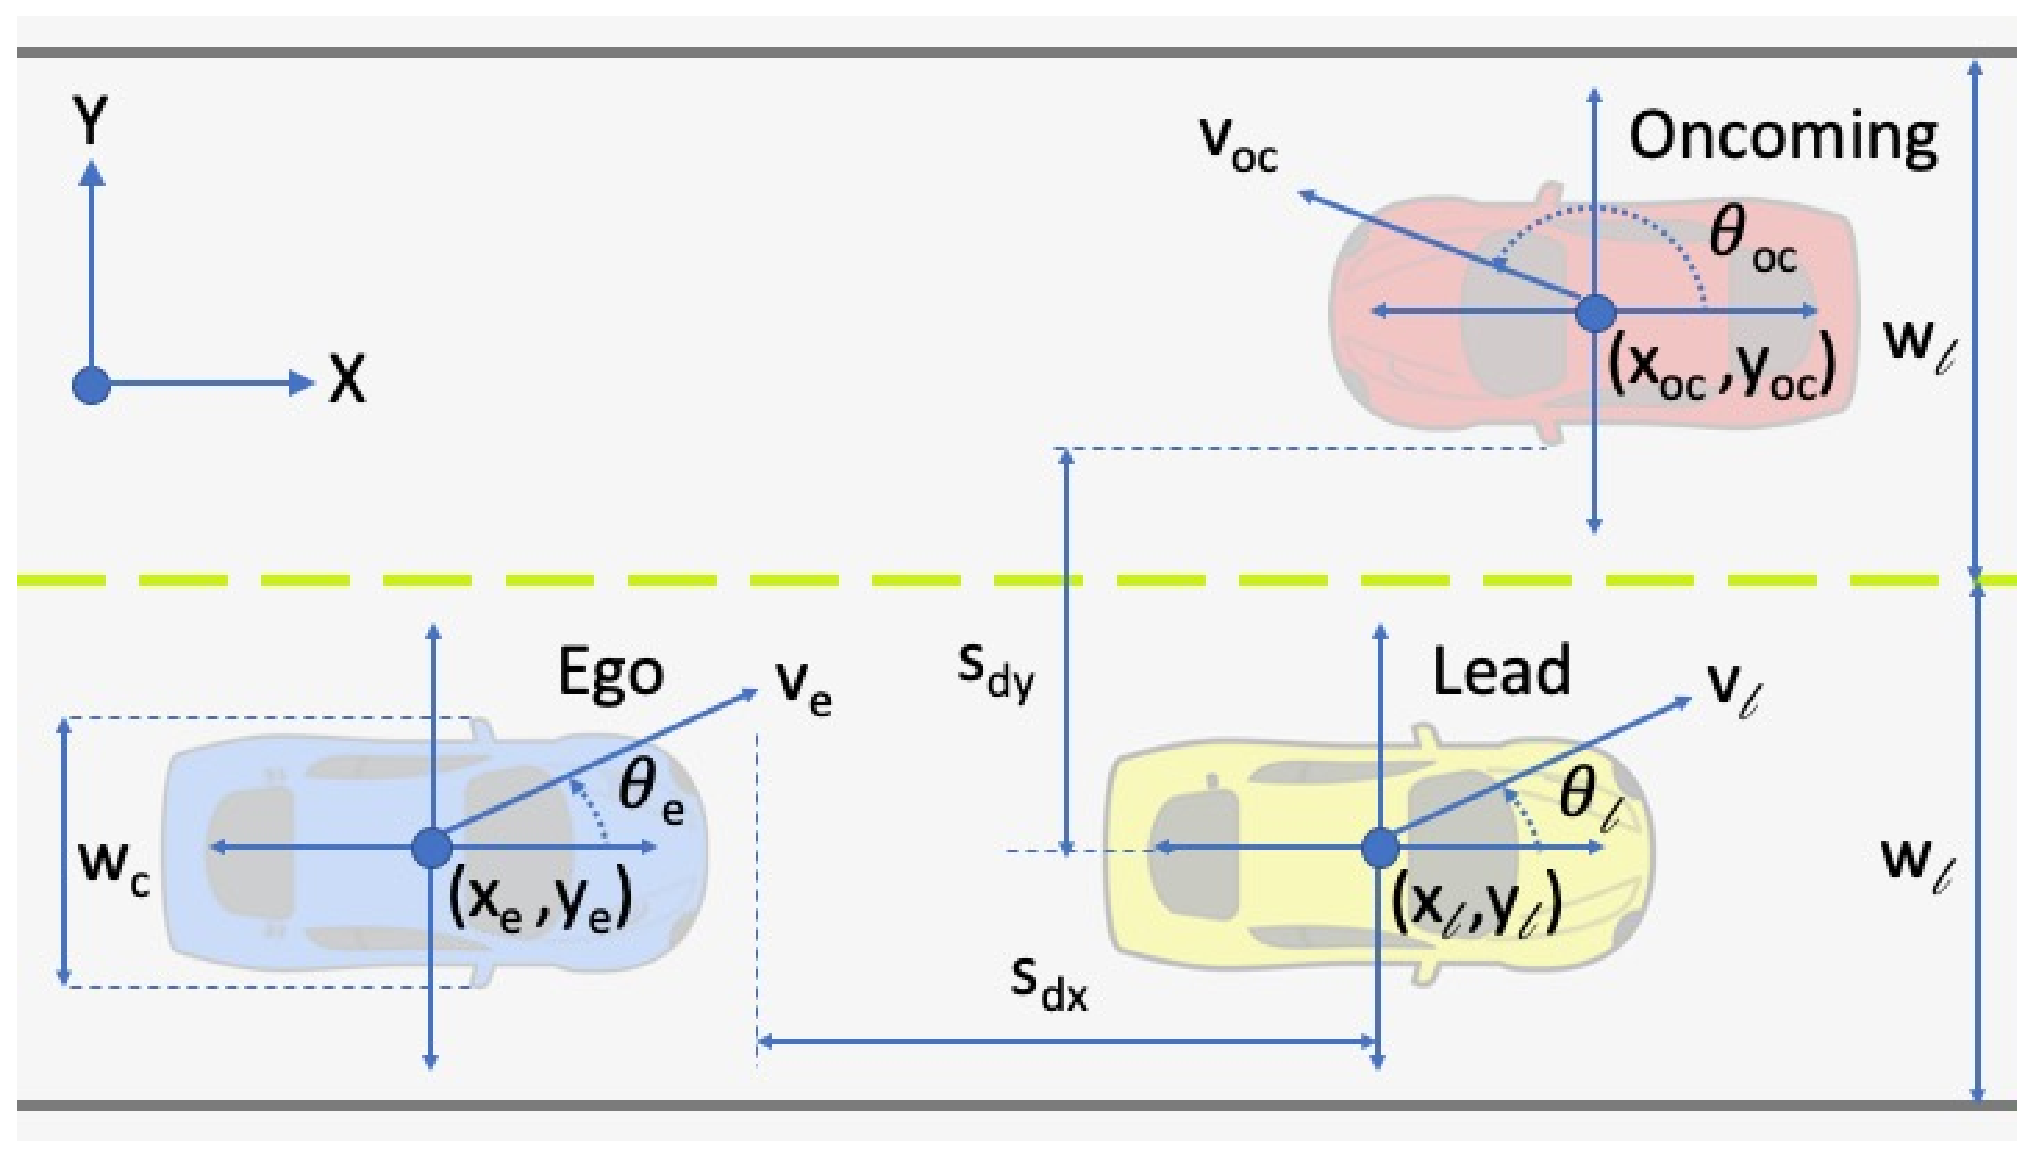
\includegraphics[width=1\columnwidth,clip]{ProblemDescription.eps}
%     \caption{Problem setup for the overtake problem.}\label{fig:problem setup}
% \end{figure}

% For each vehicle, we select the model of a kinematic bicycle in an inertial frame, introduced in \cite{Rajamani2012VDC} and adapted for automobile highway merging in \cite{huang2018highwaymerging}. We use subscripts $e, l, oc$ to denote the Ego, the Lead and Oncoming car. The motion of the cars is modelled as:\small{
% \begin{align}\label{eq: overtake_dynamics}
%     \dot q_i = 
%         \begin{bmatrix}
%             v_i \ cos(\theta_i) \\
%             v_i \ sin(\theta_i) \\
%             0 \\  0
%         \end{bmatrix}
%         + 
%         \begin{bmatrix}
%             0 & 0 \\
%             0 & 0 \\
%             1 & 0 \\
%             0 & 1
%         \end{bmatrix}
%         \begin{bmatrix}
%             \omega_i \\ a_i\end{bmatrix}+ \phi_i,
% \end{align}}\normalsize
% where $q_i = [x_i \ y_i \ \theta_i \ v_i]^T$ is the state vector of car $i\in \{e, l, oc\}$, $x_i$ is the longitudinal position, $y_i$ is the transverse position, $\theta_i$ is the heading angle, $v_i$ is the velocity of car $i$, $\omega_i$ is the angular control input, and $a_i$ is the longitudinal control input (measured as a fraction of $M_ig$, where $M_i$ is the mass of vehicle $i$ and $g = 9.81$ m/s$^2$). {\color{blue}The considered disturbance in the Ego car's dynamics $\phi_e = \phi_e(q_e, q_l, q_{oc})$, among other things, models measurement uncertainties as well as errors in the states of the Lead and Oncoming vehicle as measured by the Ego car.} {\color{blue}We assume that the disturbance $\phi$}, and thus, the measurement error is bounded, i.e., if $\hat q_l^e, \hat q_{oc}^e$ denote the states of the Lead and Oncoming car as estimated by Ego car, then there exists $\epsilon>0$ such that $\|\hat q_j^e(t)-q_j(t)\|\leq \epsilon$ for all $t\geq 0$, $j \in \{l, oc\}$. Consistent with the discussion in the previous section, we define $\|\phi\|_\infty = \epsilon$.

% The control input $u_i\in \mathbb R^2$ for car $i$ consists of $\omega_i$ and $a_i$. Notably, our adjustment to the dynamics of \cite{Rajamani2012VDC} is such that $\theta$ describes the full steering dynamics, $\theta = \frac{v\tan(\beta)}{l_v}$, where $\beta$ is the steering angle in rad and $l_v$ is the length of the vehicle in m. This is a reasonable modification due to the small angle approximation, which we expect to hold in our overtaking problem, and from which we obtain that $tan(\beta) \approx \beta$, such that $\theta \approx \frac{v\beta}{l_v}$. Additionally, it is important to note that although the vehicles are now effectively point masses, they still obey the no-slip condition imposed by the kinematic bicycle model; moreover, we take vehicle width and length into consideration when evaluating safety. 

% The overtake problem considered in the case study is formally stated below.

% \begin{Problem}\label{Prob: Automobile Overtake}
% \end{Problem}

% The CBFs $h_{s,i}(q)$ were defined as follows:
% \begin{align}
%     h_{s,1} & = (y_e - e_1)(y_e - e_2)\\
%     h_{s,2} & = 1 - (\frac{x_{l} - x_e}{s_{dx}})^2 - (\frac{y_{l} - y_e}{s_{dy}})^2&&
% \end{align}
% where $s_{dx} = v_e \tau \cos{\theta _e} + l_c$ is the safe-distance in x-coordinates between vehicles, $s_{dy} = w_l - \frac{w_c}{2}$ is safe-distance in y-coordinates between vehicles, and $e_1$, $e_2$ are parameters which define the safety barrier at the edge of the road in the $y$ coordinate. Here, $\tau = 1.8$ sec is the time headway\footnote{The selection of $\tau = 1.8$ sec comes from the "half-the-speedometer" rule, as in \cite{xu2015robustness}.}.  
% Specifically, we define $e_1 = (\frac{w_c}{2}) + v_e\omega _{max}\left(1 - \cos{\theta _e}\right)$, and $e_2 = (2w_l - \frac{w_c}{2}) - v_e\omega _{max}\left(1 - \cos{\theta _e}\right)$, where $w_l = 3$m is the width of a lane\footnote{Taken from \url{https://tinyurl.com/knzhwje}} and $w_c = 2.27$m and $l_c = 5.05$m are the width and length of a car\footnote{Taken from \url{ https://tinyurl.com/tqyhqxr}}. 

% To capture the convergence requirement in each of the sub-problems 2) -- 4), we define goal sets $S_j = \{q\; |\; V(q-q_j^g)\leq 0\}$, where $q_j^g = [x_j^g\; y_j^g\; \theta_j^g\;v_j^g]^T$ denotes the goal location for the $j-th$ sub-problem, $j\in \{2, 3, 4\}$, and we define $\bar q_j = q-q_j^g$. We use a CLF $V:\mathbb R^4\rightarrow\mathbb R$ to encode the convergence requirement, defined as
% \begin{align}\label{ex: CLF}
% \begin{split}
%     V(\bar q) = & K (k_x\bar x^2 + k_v\bar v^2 + k_{xv}\bar x\bar v \\ & + k_y\bar y^2 + k_\theta\bar \theta^2 + k_{y\theta}\bar y\bar \theta -1)\\
% \end{split}
% \end{align}
% where $K$ is a constant gain selected during our parameter selection phase, $k_x$, $k_y$, $k_\theta$, $k_v$, $k_{xv}$, $k_{y\theta}$ are constant gains which influence the size and shape of the goal subspace, and $\bar x =x_e-x_j^g,\bar y = y_e-y_j^g,\bar \theta = \theta_e-\theta_j^g$ and $\bar v =v_e-v_j^g$. Note that the convergence requirement, and thus the CLF $V$, changes for each sub-problem, but that $V$ is nevertheless positive definite via the geometric mean inequality.

% We will now introduce a QP formulation to solve Problem \ref{Prob: Automobile Overtake}. Consider the QP:
% \begin{subequations}\label{Robust FxT CLF-CBF QP}
% \begin{align}
%     \min_{u,\delta _1,\delta _2,\delta _3} \frac{1}{2}u^{T}u +p_1\delta _1^2 &+ p_2\delta _2^2 +p_3\delta _3^2 +q_1\delta _1 \label{pt_J}\\
%     \textrm{s.t.} \; A_{u}u & \leq b_u \label{pt_c}\\
%     L_fV(q_e)+L_gV(q_e)u & \leq  \delta _1 - \alpha_1 \max\{0,V(q_e)\}^{\gamma _1} \nonumber \\ 
%     &\quad - \alpha_2\max\{0,V(q_e)\}^{\gamma _2} \label{pt_V}\\
%     L_fh_{s_1}(q_e)+L_gh_{s_1}(q_e)u & \leq \delta _2h_{s_1}(q_e) \label{pt_S1}\\
%     L_fh_{s_2}(q_e)+L_gh_{s_2}(q_e)u & \leq \delta _3h_{s_2}(q_e) \label{pt_S2}
% \end{align}
% \end{subequations}
% where ($\ref{pt_J}$) models a minimum-norm controller with relaxation variables $\delta _1$, $\delta _2$, $\delta _3$ and $p_1$, $p_2$, $p_3$, $q_1$ $\geq 0$, $\gamma _1 = 1 + \frac{1}{\mu}$, $\gamma _2 = 1 - \frac{1}{\mu}$, where $\mu > 1$, and $\alpha _i = \frac{\pi\mu}{2T}$ for $i = \{1,2\}$. The constraint ($\ref{pt_c}$) enforces input constraints, ($\ref{pt_V}$) provides the FxT Convergence guarantee, ($\ref{pt_S1}$) and ($\ref{pt_S2}$) provide safety guarantees. Our formulation, specifically ($\ref{pt_V}$), utilizes the result of Theorem \ref{Th: FxTS new nonvan} in order to guarantee fixed-time convergence for any $\delta _1$. Moreover, we discuss the relationship between this $\delta _1$ term and an upper limit on the class of additive, bounded, non-vanishing disturbances considered in Problem \ref{Prob: Automobile Overtake}. 
% Consider the following inequalities.
% \begin{align}
%     L_fh_{s_1}(x)+L_gh_{s_1}(x)u& \leq 0, \label{eq: assum safety S1}\\
%     L_fh_{s_2}(x)+L_gh_{s_2}(x)u& \leq 0, \label{eq: assum safety S2}
% \end{align}
% which when true at the boundary of the sets $S_{s_1}$ and $S_{s_2}$ guarantee forward invariance of the respective sets. We need the following viability assumption before we can proceed with our main results. 

% \begin{Assumption}\label{Assum feas}
% There exists a control input $u\in \mathcal U$ such that 
% \begin{itemize}
%     \item[1)] for all $q\in \partial S_{s_1}\cap \partial S_{S_2}$, both \eqref{eq: assum safety S1} and \eqref{eq: assum safety S2} holds;
%     \item[2)] for all $q\in \partial S_{s_1}$ (respectively, $q\in \partial S_{s_2}$, \eqref{eq: assum safety S1} (respectively, \eqref{eq: assum safety S2}) holds.
% \end{itemize}
% Furthermore, $S_G\cap S_{s_1}\cap S_{s_2}\neq \emptyset$. 
% \end{Assumption}

% \noindent First, we discuss the feasibility of the QP \eqref{Robust FxT CLF-CBF QP}.

% \begin{Lemma}
% Under Assumption \ref{Assum feas}, the QP \eqref{Robust FxT CLF-CBF QP} is feasible for all $q\in (S_{S_1}\cap S_{S_2})\setminus S_G$.
% \end{Lemma}


%%%%%%%%%%%%%%%%%%%%%%%%%%%%%%%%%%%%%%%%%%%%%%%%%%%%%%%%%%%%%%%%%%%%%%%%%%%%%%%%
%**************************** Numerical Case Study ****************************%
%%%%%%%%%%%%%%%%%%%%%%%%%%%%%%%%%%%%%%%%%%%%%%%%%%%%%%%%%%%%%%%%%%%%%%%%%%%%%%%%

\section{Simulation Results and Discussion}\label{sec: results}

\subsection{Simulation Parameters}

\subsection{Results}

% \begin{figure}[!ht]
%     \centering
%         \includegraphics[width=1\columnwidth,clip]{nominal_trajectories.eps}
%         \includegraphics[width=1\columnwidth,clip]{nominal_inputs.eps}
%         \includegraphics[width=1\columnwidth,clip]{nominal_CLFCBF.eps}
%     \caption{Ego Vehicle trajectories, control inputs, and CLF / CBF evolution for 7 different initial conditions.}\label{fig:2}
% \end{figure}


%%%%%%%%%%%%%%%%%%%%%%%%%%%%%%%%%%%%%%%%%%%%%%%%%%%%%%%%%%%%%%%%%%%%%%%%%%%%%%%%
%********************************* Conclusion *********************************%
%%%%%%%%%%%%%%%%%%%%%%%%%%%%%%%%%%%%%%%%%%%%%%%%%%%%%%%%%%%%%%%%%%%%%%%%%%%%%%%%

\section{Conclusion}
\noindent Conclusion belongs here.
% \noindent In this study on robust control synthesis using CLF- and CBF-based techniques for safety-critical control problems, we introduced a new approach to driving a dynamical system subject to spatiotemporal and input constraints to a neighborhood of a goal set in fixed-time despite the presence of bounded, additive, non-vanishing disturbances. We provided theoretical guarantees of fixed-time convergence for such a system whose control is computed by a FxT-CLF-CBF QP provided that disturbances do not exceed a quantified bound. Next, we outlined a procedure for conditioning the QP and selecting parameters such that FxT convergence to a neighborhood of a goal set is guaranteed for any initial condition, and presented definitions for such a neighborhood. We then demonstrated the procedure on an overtake problem and highlighted the efficacy of the method with repeated simulated trials.

% In the future, we plan to investigate the relationship between QP formulations and theoretical guarantees on FxT stabilizability in the presence of bounded disturbances. Though in this work we demonstrated the utility of constructing a bound on an additive disturbance via QP parameters and using it to solve a perturbed overtake problem, we hope in future work to study the intrinsic relationship between bounds on FxT CLF-CBF QP slack variables and associated tolerable disturbances.

\bibliographystyle{IEEEtran}
\bibliography{myreferences}


%%%%%%%%%%%%%%%%%%%%%%%%%%%%%%%%%%%%%%%%%%%%%%%%%%%%%%%%%%%%%%%%%%%%%%%%%%%%%%%%
%********************************* Appendices *********************************%
%%%%%%%%%%%%%%%%%%%%%%%%%%%%%%%%%%%%%%%%%%%%%%%%%%%%%%%%%%%%%%%%%%%%%%%%%%%%%%%%

\appendices
\section{Proof of Something}
App. 1.

\end{document}